\FloatBarrier

\section{Appendix: The SMS cases}
\label{app:smscases}
In this appendix, details about the SMS cases are given, split up by the
production mechanism.

\subsection{The ``gluinos'' case}
\label{ssec:gluinocase}
The case of gluino-gluino production is the richest in terms of experimental results:
Fig.~\ref{fig:gluinoSMSes} shows the Feynman graphs of all processes that can be covered by LHC results, Tab.~\ref{tab:classgluinos} lists how all SMSes are identified, and what results have been applied.

\begin{figure}[h!t]
\begin{center}
\begin{tabular}{lcr}
\subfigure[\label{fig:T1}T1]{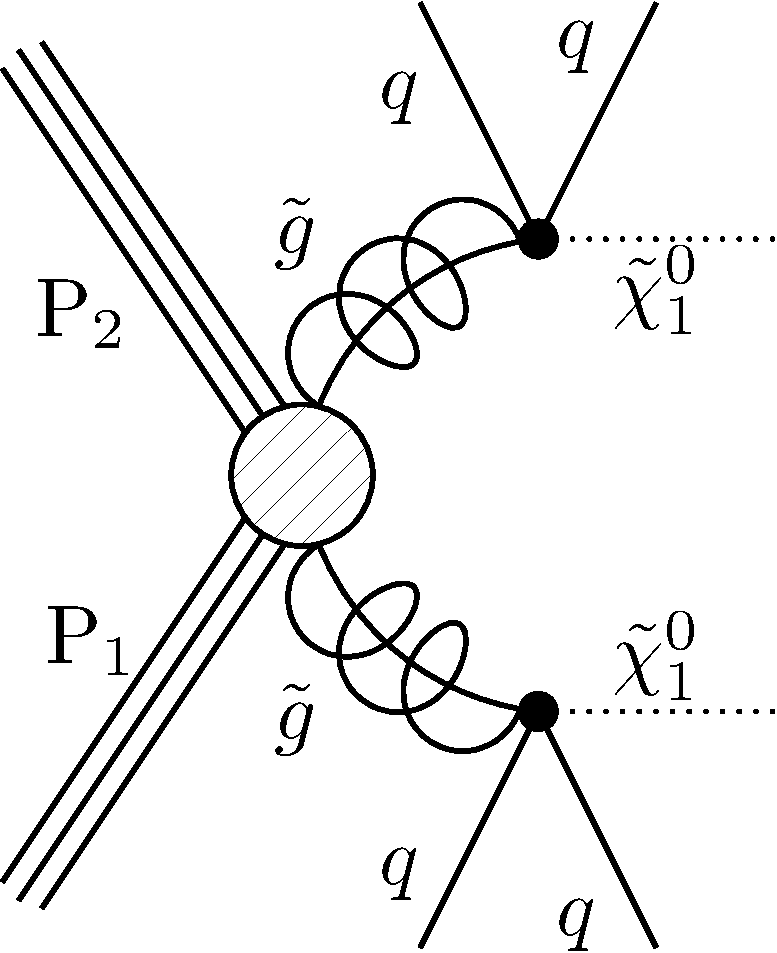
\includegraphics[width=0.2\linewidth]{figures/T1_feyn.pdf}}\spacer &
\subfigure[\label{fig:T3w}T3w]{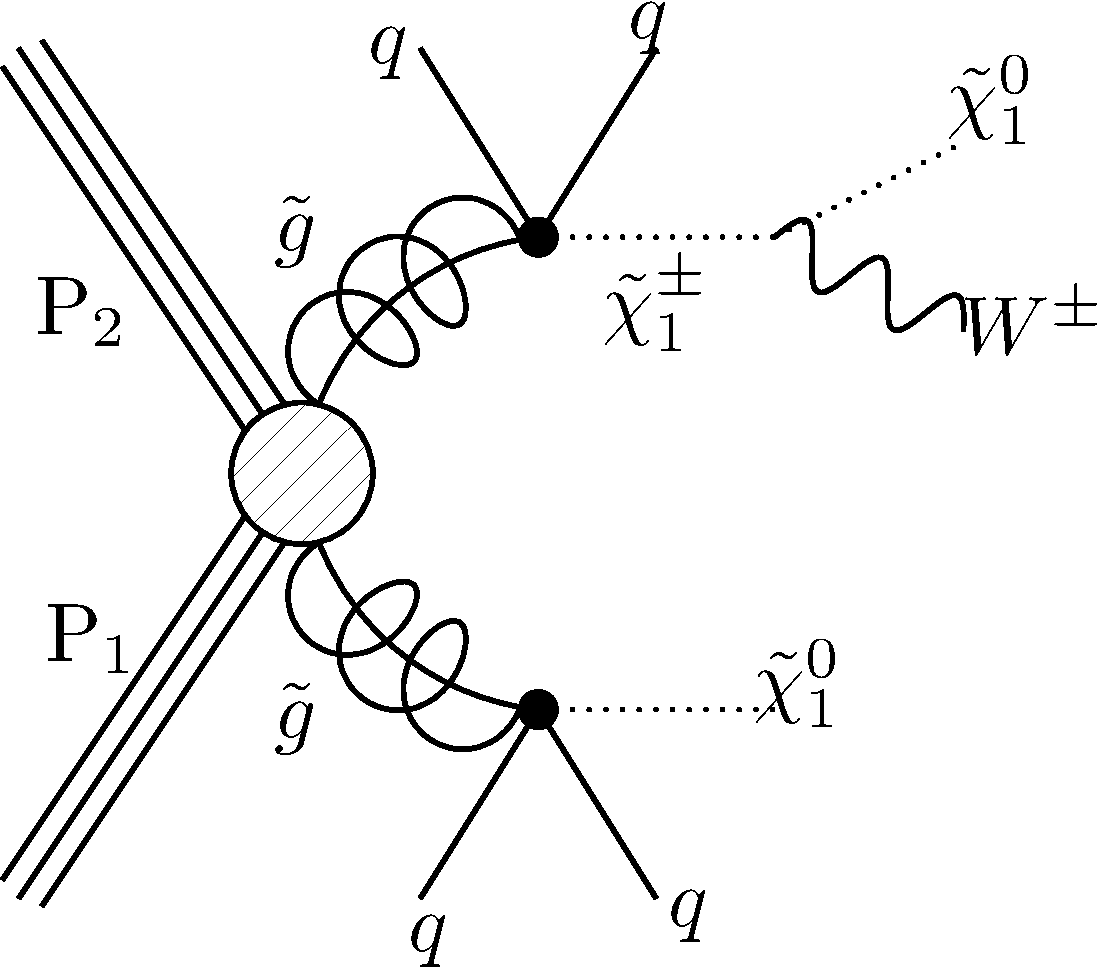
\includegraphics[width=0.26\linewidth]{figures/T3w_feyn.pdf}}\spacer &
\subfigure[\label{fig:T3C}T3C]{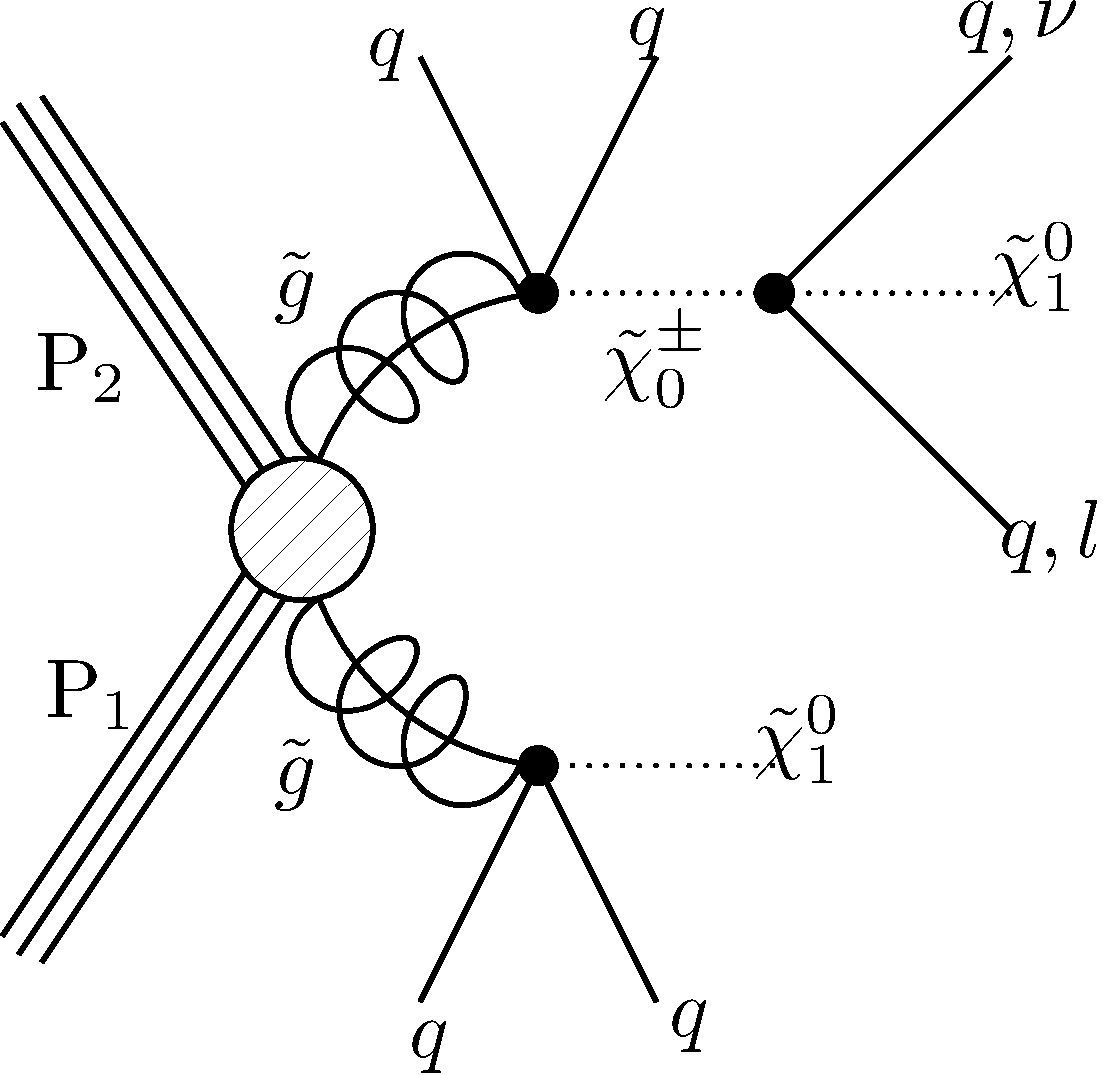
\includegraphics[width=0.26\linewidth]{figures/T3C_feyn.pdf}}\spacer \\
\subfigure[\label{fig:T5zz}T5zz]{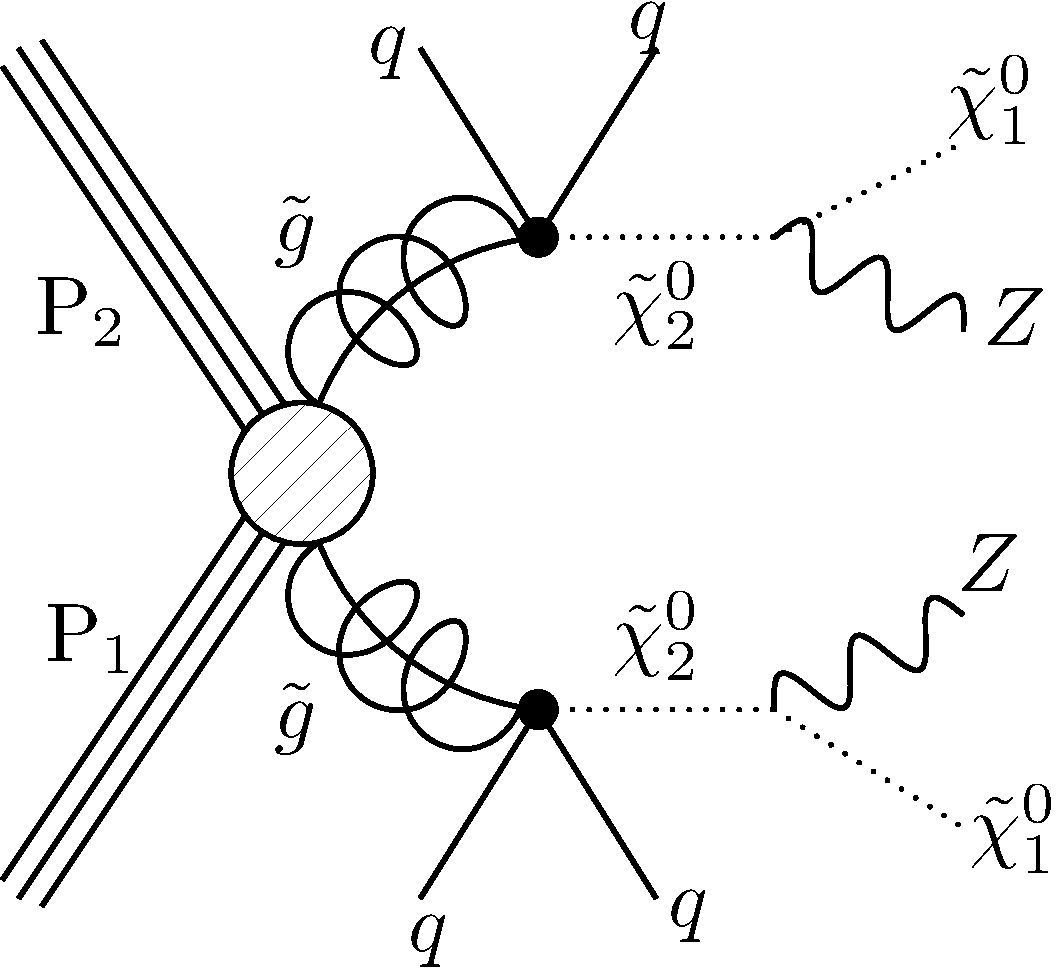
\includegraphics[width=0.26\linewidth]{figures/T5zz_feyn.pdf}} \spacer &
\subfigure[\label{fig:T5qqqq}T5qqqq]{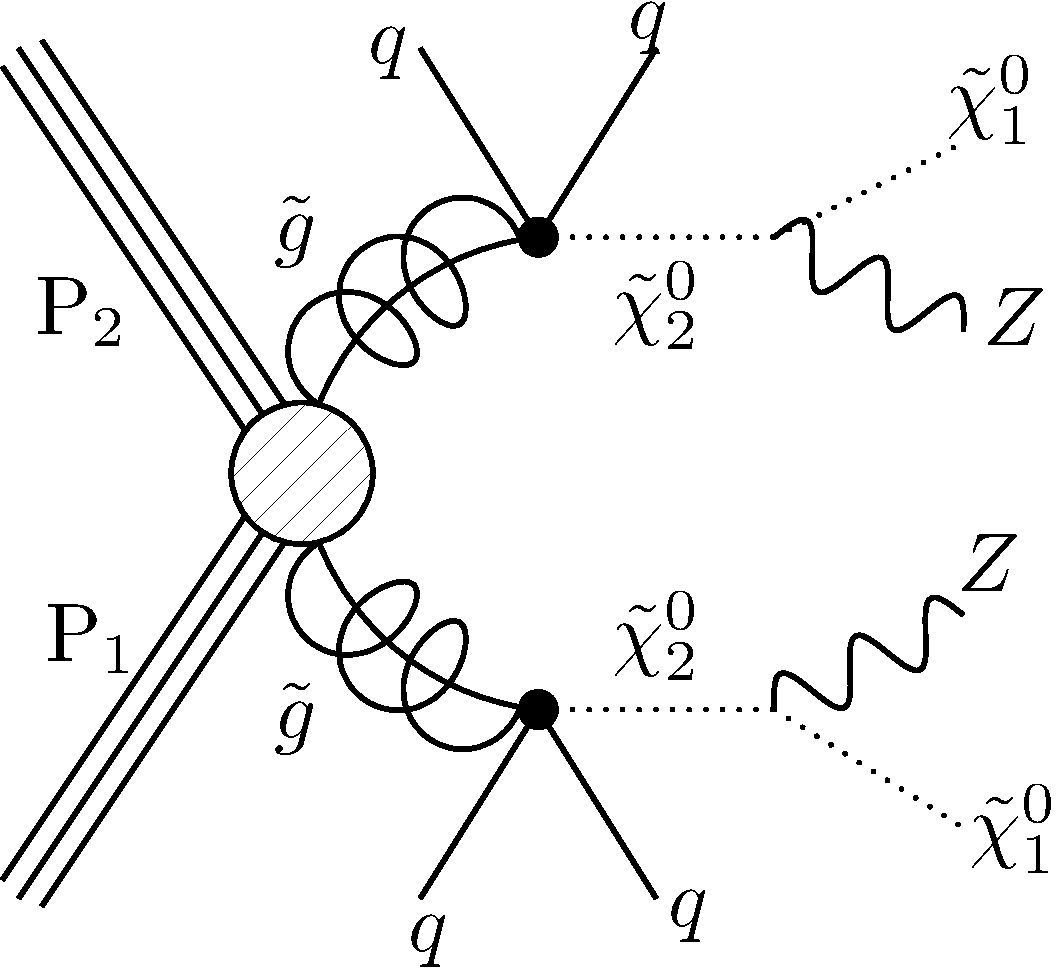
\includegraphics[width=0.26\linewidth]{figures/T5zz_feyn.pdf}} \spacer \\
% \subfigure[\label{fig:T5ww}T5ww]{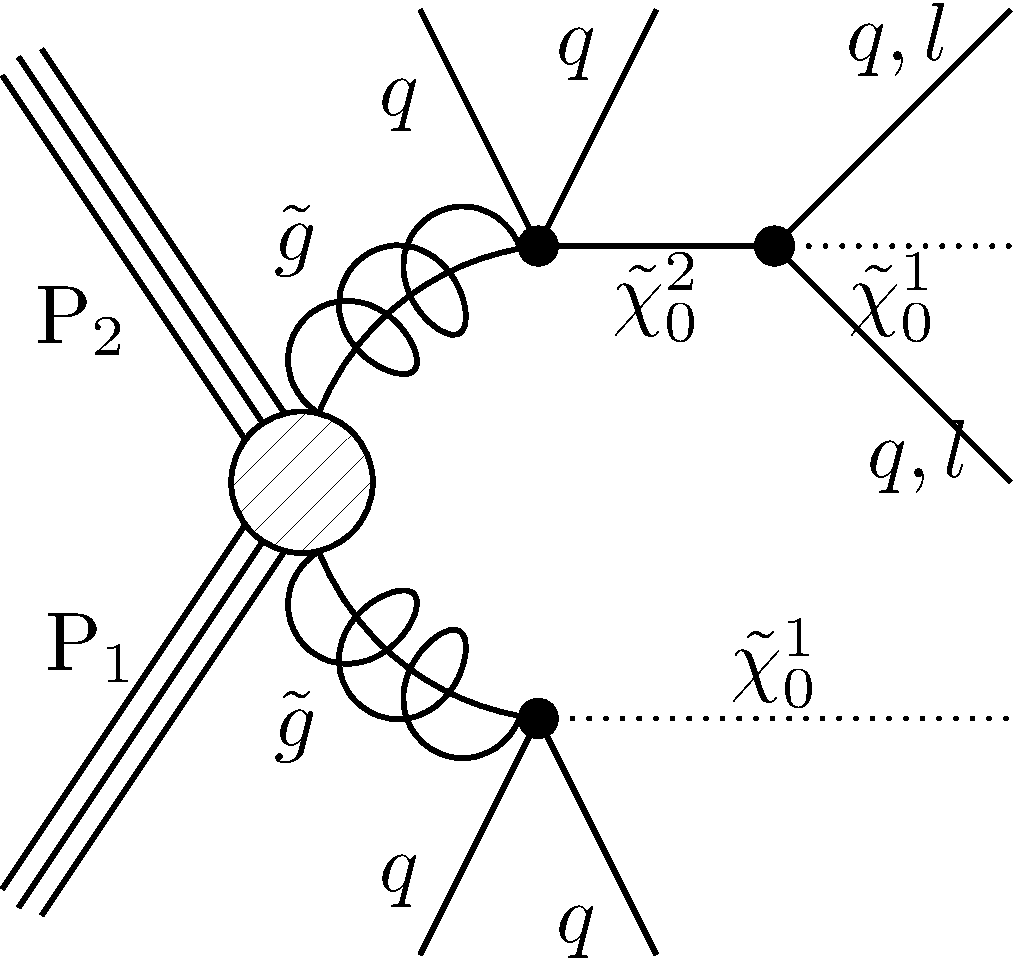
\includegraphics[width=0.2\linewidth]{figures/T3N_feyn.pdf}} \spacer \\
\end{tabular}
\caption{A few simplified models for gluino-gluino production. \fixme{Once we know what models we use, we choose more appropriate models. need to (re)draw a few plots: T3C, T5qqqq}}
\label{fig:gluinoSMSes}
\end{center}
\end{figure}

\begin{table}[h!]\centering
\begin{tabular}{|c|c|c|c|c|c|}
\hline
additional & & & & & Results \\
particle content & Production & Decay & SMS & Figure & from \\
\hline
qqqq & $\gl \rightarrow qq\chiz$ & & \model{T1} & Fig.~\ref{fig:T1} & \AlphaT, \HsTjets, \MTtwo, razor \\
\hline
qqqqW & $\gl \rightarrow qq\chiz$, & $\chipm\rightarrow W \chiz$  & \model{T3w}  & Fig.~\ref{fig:T3w}  & $\emu$ LS, $\emu$ LP, $\emu$ ANN  \\
 & $\gl \rightarrow qq\chipm$ & & & & \\
\hline
qqqql & $\gl \rightarrow qq\chiz$, & $\chipm\rightarrow l \nu \chiz$  & \model{T3C}  & Fig.~\ref{fig:T3C}  & $ \emu$ LS, $\emu$ LP, $\emu$ ANN \\
 & $\gl \rightarrow qq\chipm$ & & & & hadronic \model{T3w} results apply \\
\hline
qqqqZZ& $\gl \rightarrow qq\chitz$ & $\chitz\rightarrow Z \chiz$  & \model{T5zz} & Fig.~\ref{fig:T5zz} & \AlphaT, \HsTjets, \MTtwo \\
 & & &                     & & \ZMET, JZB, multileptons  \\
\hline
qqqqqqqq& $\gl \rightarrow qqqq\chiz$ & & \model{T5qqqq} & Fig.~\ref{fig:T5qqqq} & \AlphaT, \HsTjets, \MTtwo  \\
 & & &                     & & hadronic \model{T5zz} results apply\\
\hline
\end{tabular}
\caption{SMS case ``gluinos'': Classification of events with two gluinos as
SUSY mothers. ``q'' as additional particle content means any \first or \second generation quark.}
\label{tab:classgluinos}
\end{table}

\FloatBarrier

\subsection{The ``squarks'' case}
\label{ssec:squarkcase}

\begin{figure}[ht!]
\begin{center}
%\begin{tabular}{lcr}
\begin{tabular}{c}
\subfigure[\label{fig:T2}T2]{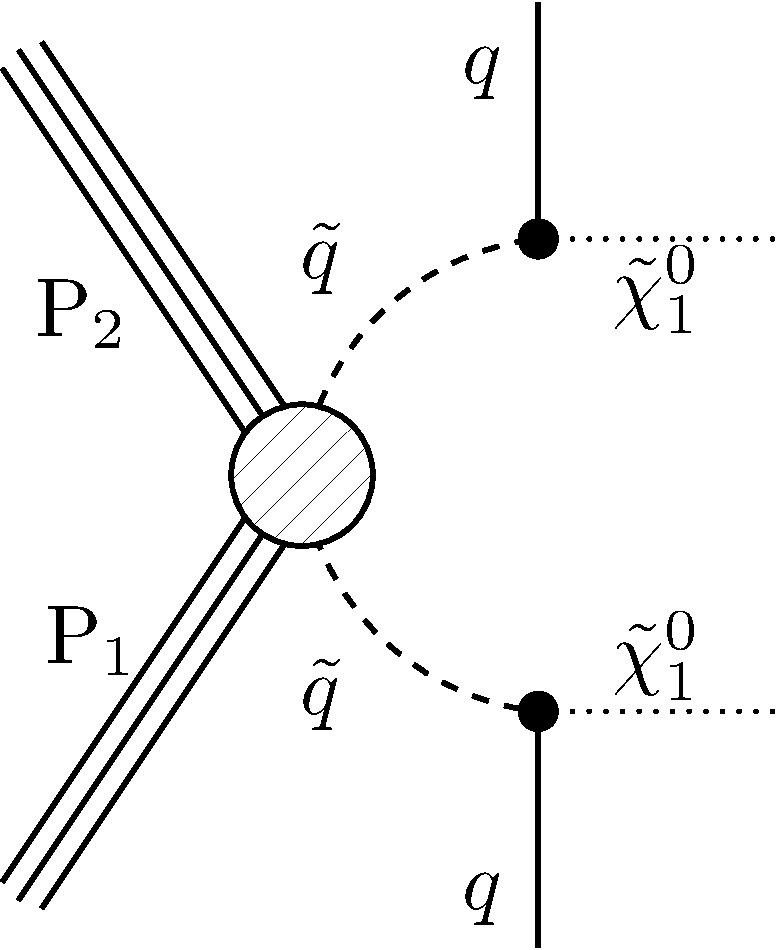
\includegraphics[width=0.2\linewidth]{figures/T2_feyn.pdf}}\spacer
%\subfigure[\label{fig:T2tt}T2tt]{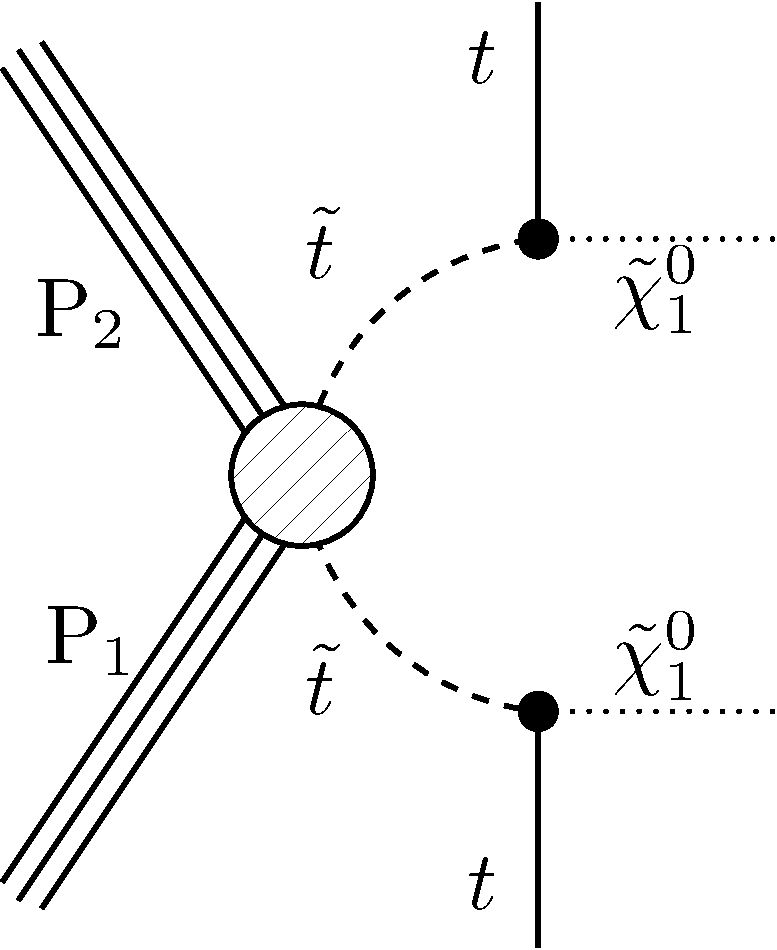
\includegraphics[width=0.2\linewidth]{figures/T2tt_feyn.pdf}}\spacer &
%\subfigure[\label{fig:T2bb}T2bb]{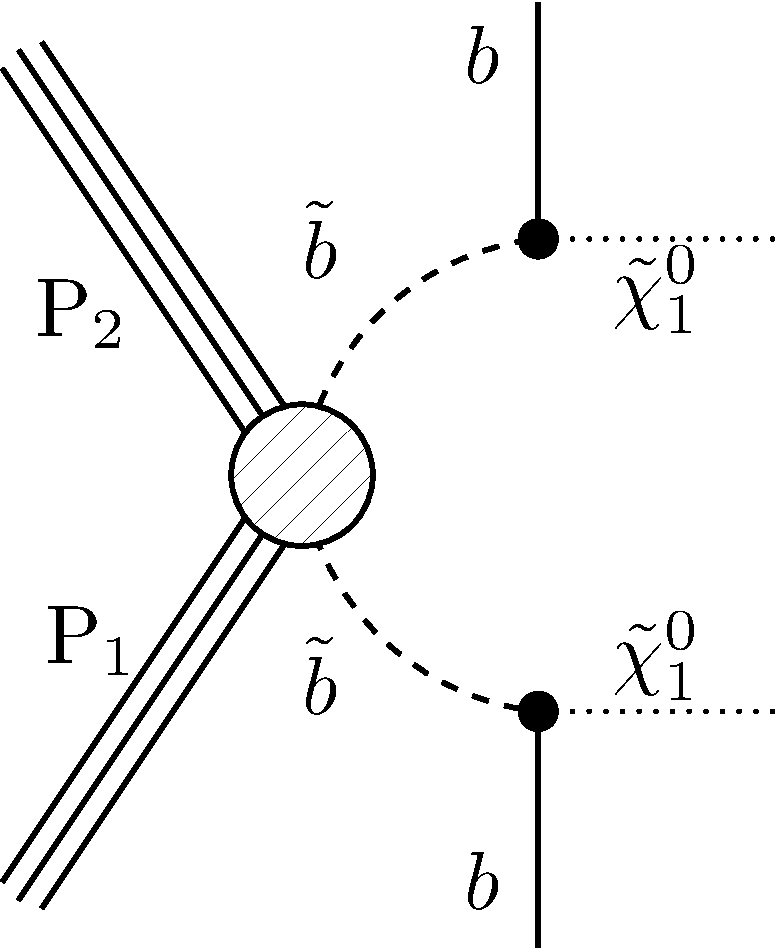
\includegraphics[width=0.2\linewidth]{figures/T2bb_feyn.pdf}}\spacer \\
\end{tabular}
\caption{A few simplified models for squark-squarkbar production. \fixme{Once we know what models we use, we choose more appropriate models.}}
\label{fig:squarkSMSes}
\end{center}
\end{figure}


\begin{table}[h!]\centering
\begin{tabular}{|c|c|c|c|c|c|}
\hline
additional & & & & & Results \\
particle content & Production & Decay & SMS & Figure & from \\
\hline
qq & $\sq \rightarrow q\chiz$ & & \model{T2} & Fig.~\ref{fig:T2} & \AlphaT, \HsTjets, razor \\
\hline
\end{tabular}
\caption{SMS case ``squarks'': Classification of events with two first or second generatiorn squarks as
SUSY mothers. ``q'' as additional particle content means any \first or \second generation quark.}
\label{tab:classsquarks}
\end{table}

\FloatBarrier

\subsection{The \third generation case}
\label{ssec:thirdcase}
Naturalness demands that both stop quarks and one sbottom quark be very light, typically below 1 TeV (\fixme{what can we cite here?}).
Both ATLAS and CMS have therefore invested major fractions of their ressources into
probing the third generation of the squark spectrum, particularly in the last two years.
Thus, a fair number of SMS results for stop and sbottom production models is
available, as can be seen in Fig.~\ref{fig:thirdSMSes}, Tab.~\ref{tab:classstops},
and Tab.~\ref{tab:classsbottoms}.

\begin{figure}[ht!]
\begin{center}
\begin{tabular}{lcr}
\subfigure[\label{fig:T2tt}T2tt]{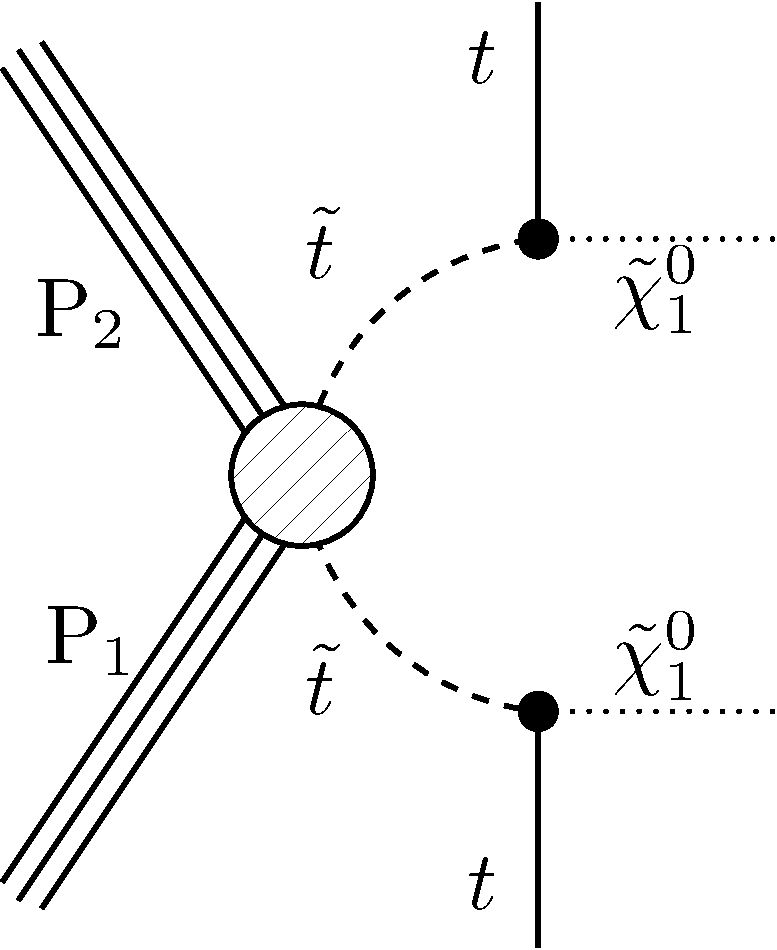
\includegraphics[width=0.2\linewidth]{figures/T2tt_feyn.pdf}}\spacer &
\subfigure[\label{fig:T6bbWW}T6bbWW]{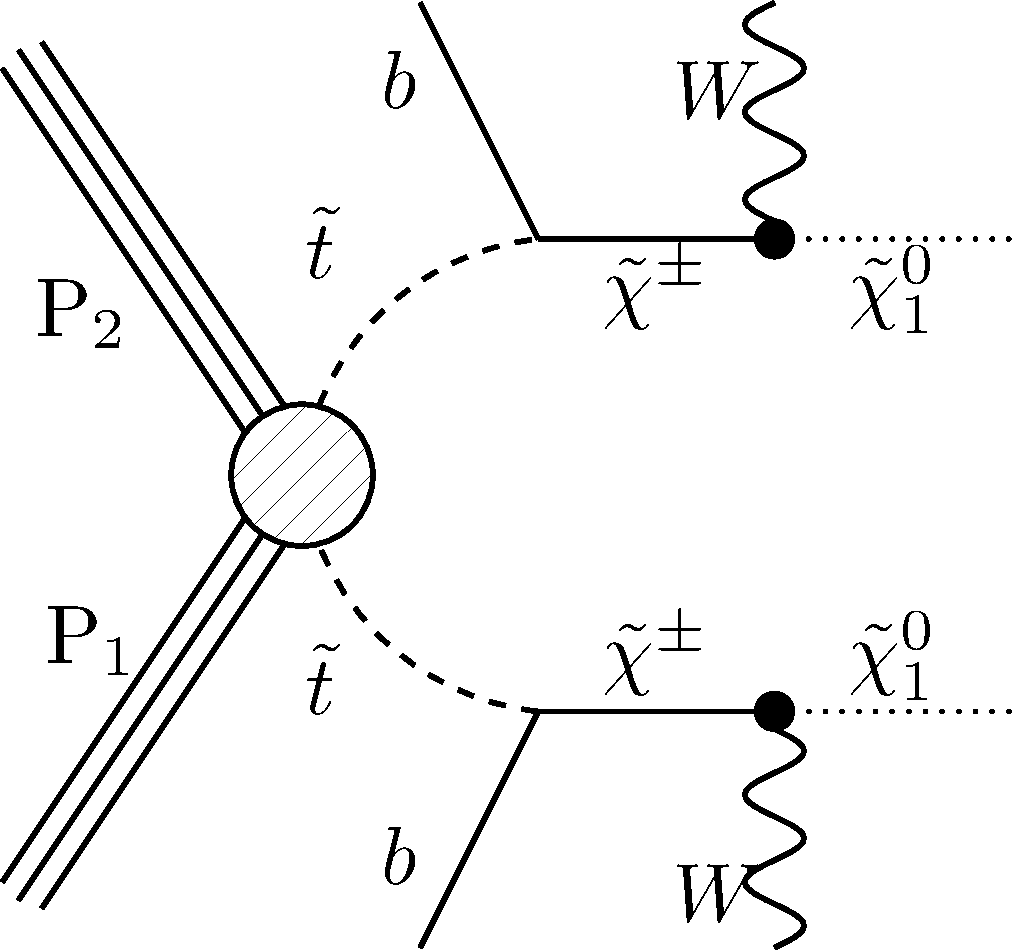
\includegraphics[width=0.26\linewidth]{figures/T6bbWW_feyn.pdf}}\spacer &
\subfigure[\label{fig:T2FVttcc}T2FVttcc]{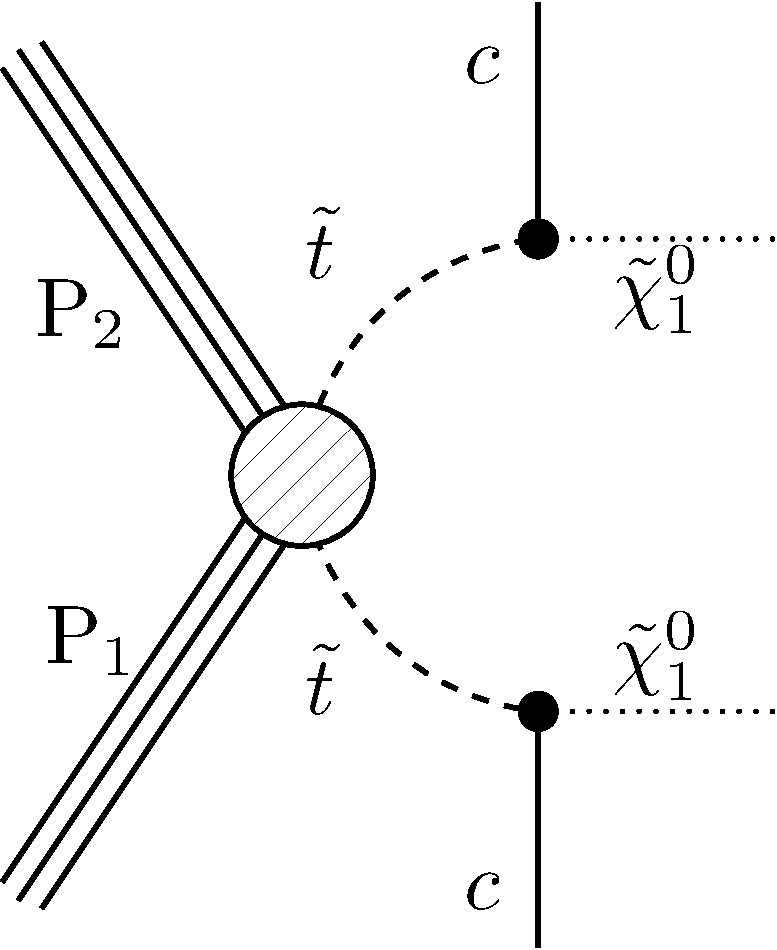
\includegraphics[width=0.2\linewidth]{figures/T2FVttcc_feyn.pdf}}\spacer \\
\subfigure[\label{fig:T2bb}T2bb]{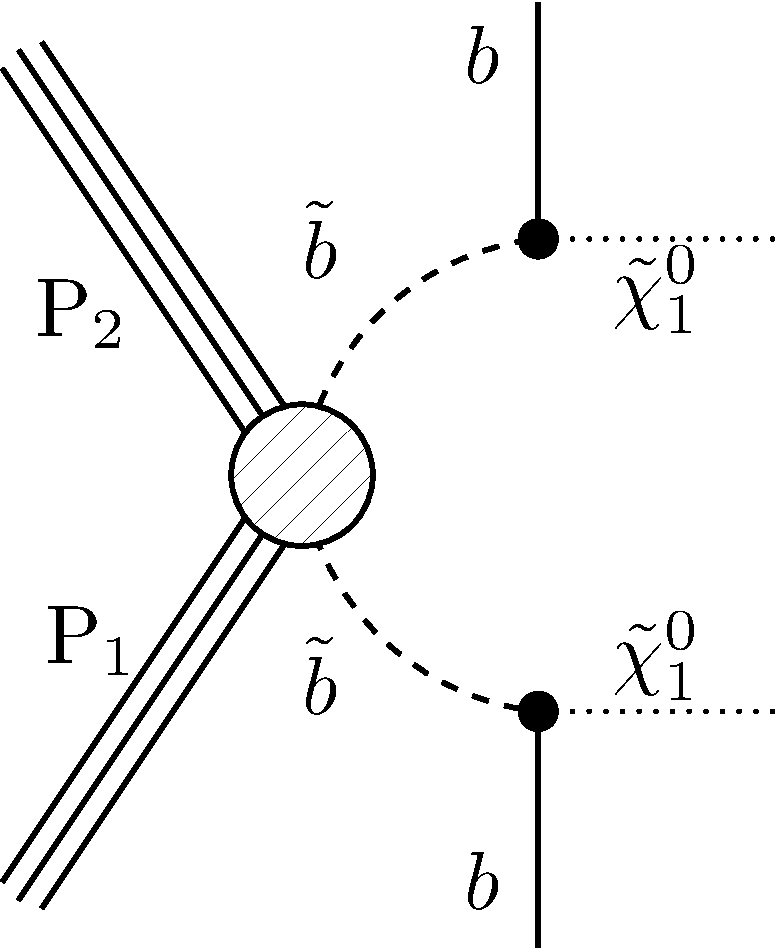
\includegraphics[width=0.2\linewidth]{figures/T2bb_feyn.pdf}}\spacer &
\subfigure[\label{fig:T6ttWW}T6ttWW]{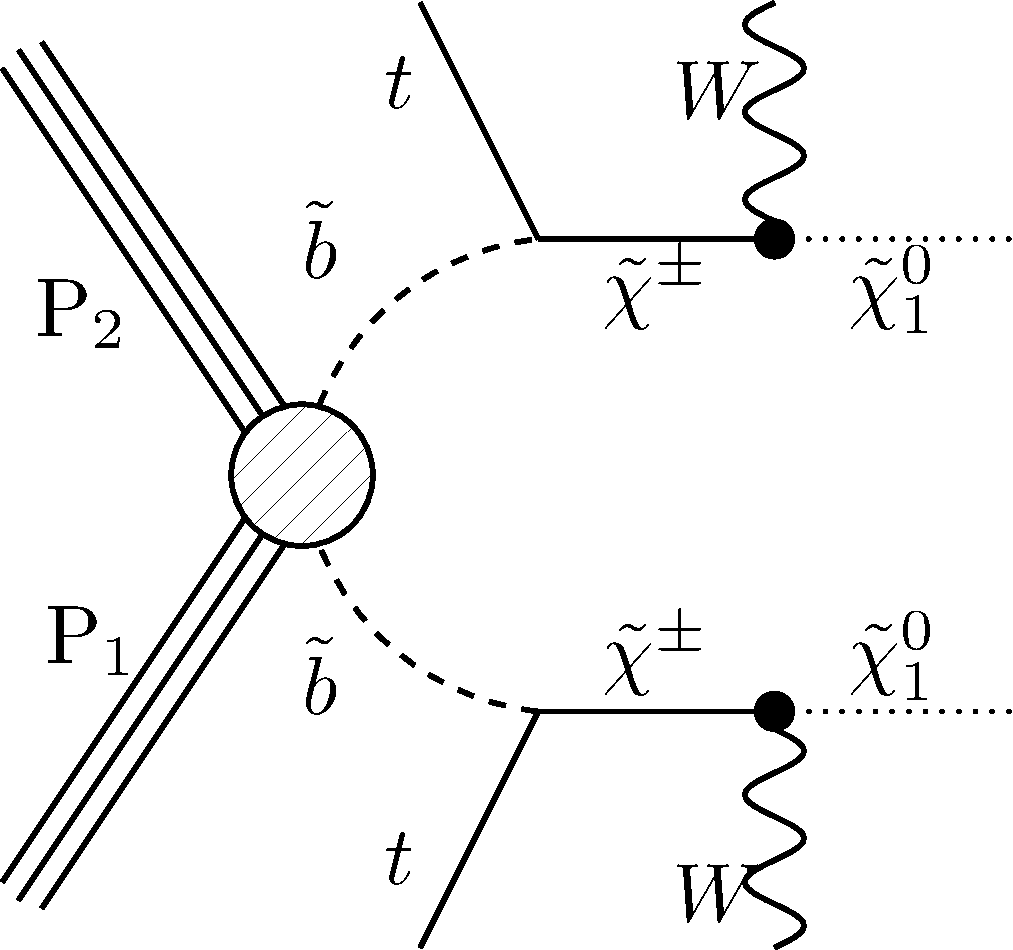
\includegraphics[width=0.26\linewidth]{figures/T6ttWW_feyn.pdf}}\spacer \\
\end{tabular}
\caption{A few simplified models for stop and sbottom production. \fixme{Once we know what models we use, we redo this list.}}
\label{fig:thirdSMSes}
\end{center}
\end{figure}


\begin{table}[h!]\centering
\begin{tabular}{|c|c|c|c|c|c|}
\hline
additional & & & & & Results \\
particle content & Production & Decay & SMS & Figure & from \\
\hline
tt & $\sTop \rightarrow t\chiz$ & & \model{T2tt} & Fig.~\ref{fig:T2tt} & razor, razor+b, razor+jets,  \\
                           & & & & & \AlphaT, hadronic \sTop, leptonic \sTop, \\
                           & & & & & \ATLLepStop \\
\hline
$bb\chipm\chipm$WW & $\sTop \rightarrow b\chipm$ & $\chipm \rightarrow W \chiz$ & \model{T6bbWW} & Fig.~\ref{fig:T6bbWW} & \ATLLepStop, \ATLHadStop \\
\hline
cc & $\sTop \rightarrow c\chiz$ & & \model{T2FVttcc} & Fig.~\ref{fig:T2FVttcc} & alphaT8TeV \\
   &  & &    & & monojets8, razormono8 \\
\hline
\end{tabular}
\caption{SMS case ``stops'': Classification of events with two top squarks as SUSY mothers}
\label{tab:classstops}
\end{table}

\begin{table}[h!]\centering
\begin{tabular}{|c|c|c|c|c|c|}
\hline
additional & & & & & Results \\
particle content & Production & Decay & SMS & Figure & from \\
\hline
bb & $\sBottom \rightarrow b\chiz$ & & \model{T2bb} & Fig.~\ref{fig:T2bb} & razor+b, \AlphaT,alphaT8 \\
\hline
ttWW & $\sBottom \rightarrow t\chipm$ & $\chipm \rightarrow W \chiz$ & \model{T6ttWW} & Fig.~\ref{fig:T6ttWW} & SS+b \\
\hline
\end{tabular}
\caption{SMS case ``sbottoms'': Classification of events with two bottom squarks as SUSY mothers}
\label{tab:classsbottoms}
\end{table}

\FloatBarrier

\subsection{Weakino production}
\label{ssec:weakinocase}
In the pMSSM, production of charginos and/or heavy neutralinos results in
cascades with only little energy; they can thus only be probed by multi-lepton
signatures, no hadronic results are available for such small mass splittings.
See Fig.~\ref{fig:weakinoSMSes} for the Feynman graphs and
Tab.~\ref{tab:classweakinos} for a list of the available results.

\begin{figure}[ht!]
\begin{center}
\begin{tabular}{lcr}
\subfigure[\label{fig:TChiwz}TChiwz]{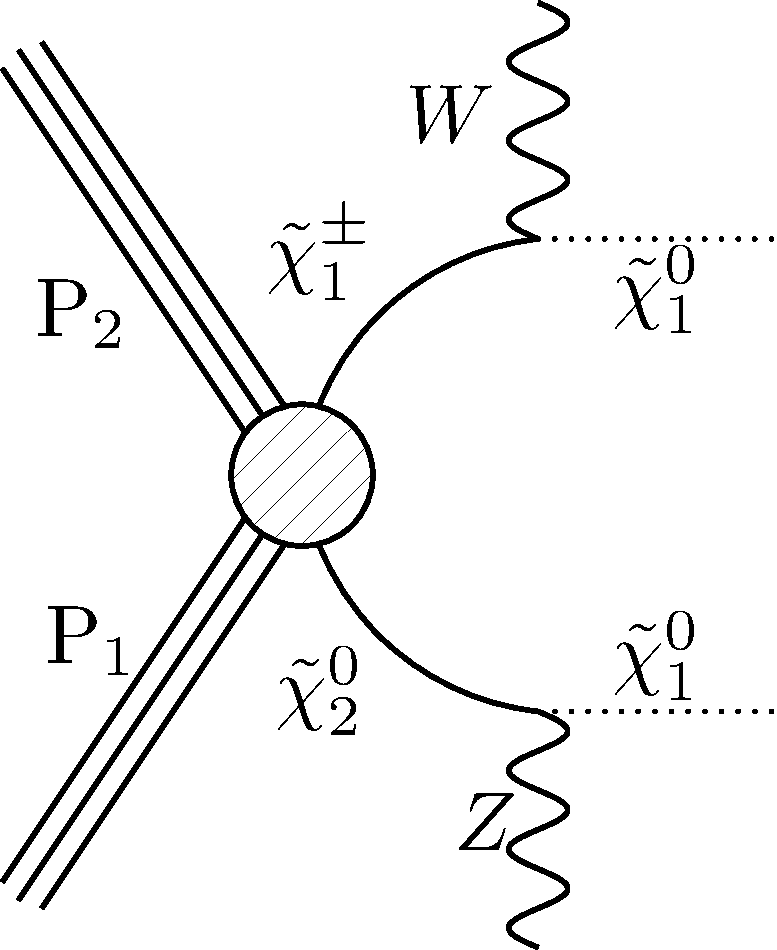
\includegraphics[width=0.2\linewidth]{figures/TChiwz_feyn.pdf}}\spacer &
\subfigure[\label{fig:TChizz}TChizz]{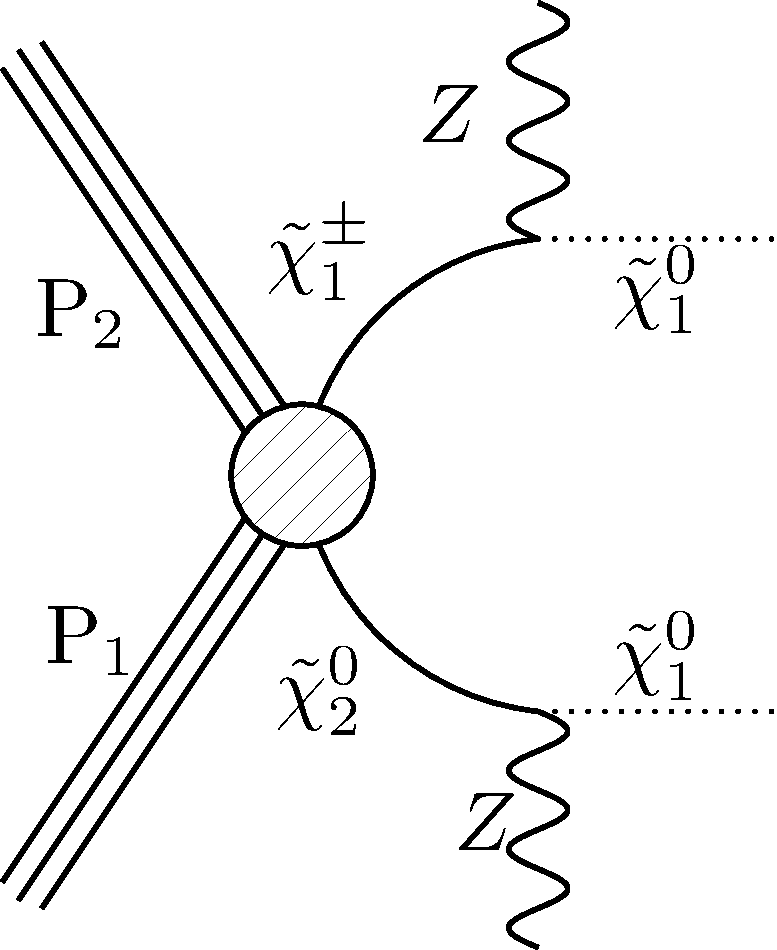
\includegraphics[width=0.2\linewidth]{figures/TChizz_feyn.pdf}}\spacer &
\subfigure[\label{fig:TChiN2C1}TChiN2C1]{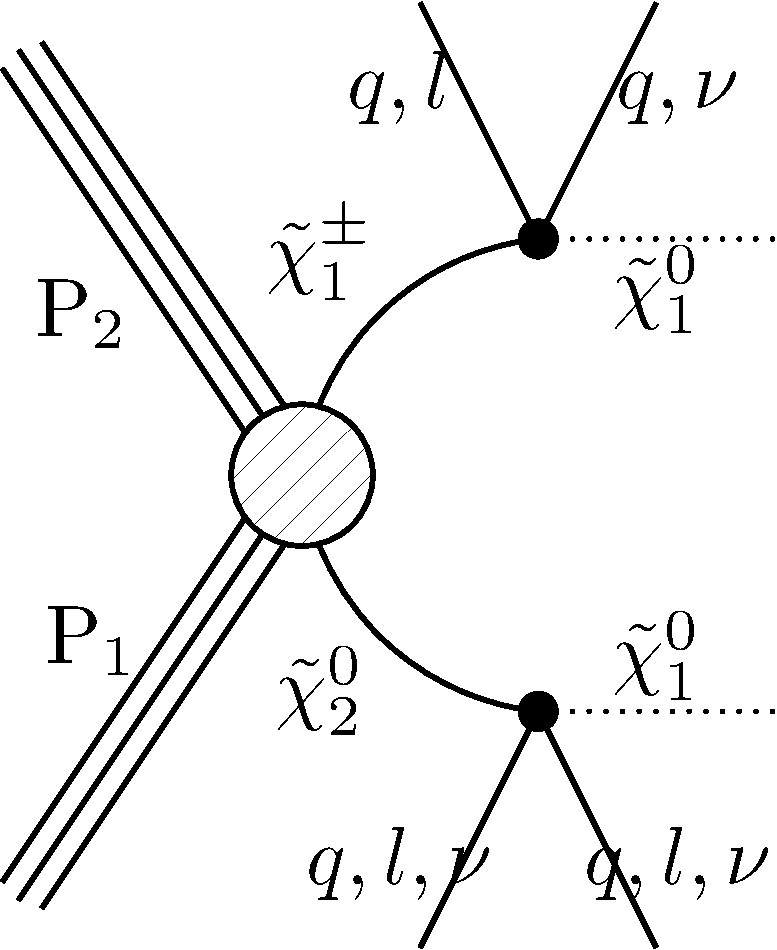
\includegraphics[width=0.2\linewidth]{figures/TChiN2C1_feyn.pdf}}\spacer \\
\subfigure[\label{fig:TChiChipmSlepSlep}TChiChipmSlepSlep]{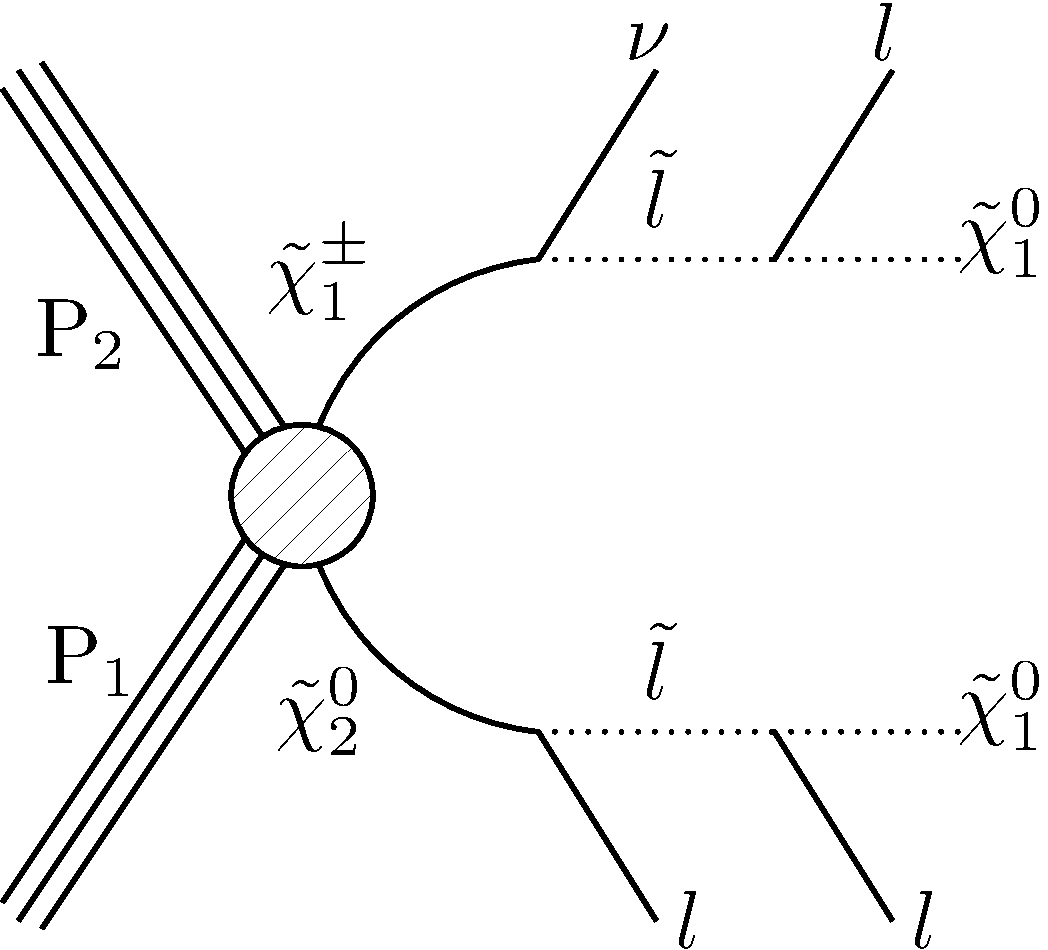
\includegraphics[width=0.26\linewidth]{figures/TChiChipmSlepSlep_feyn.pdf}}\spacer &
\subfigure[\label{fig:TChiChipmSnuSlep}TChiChipmSnuSlep]{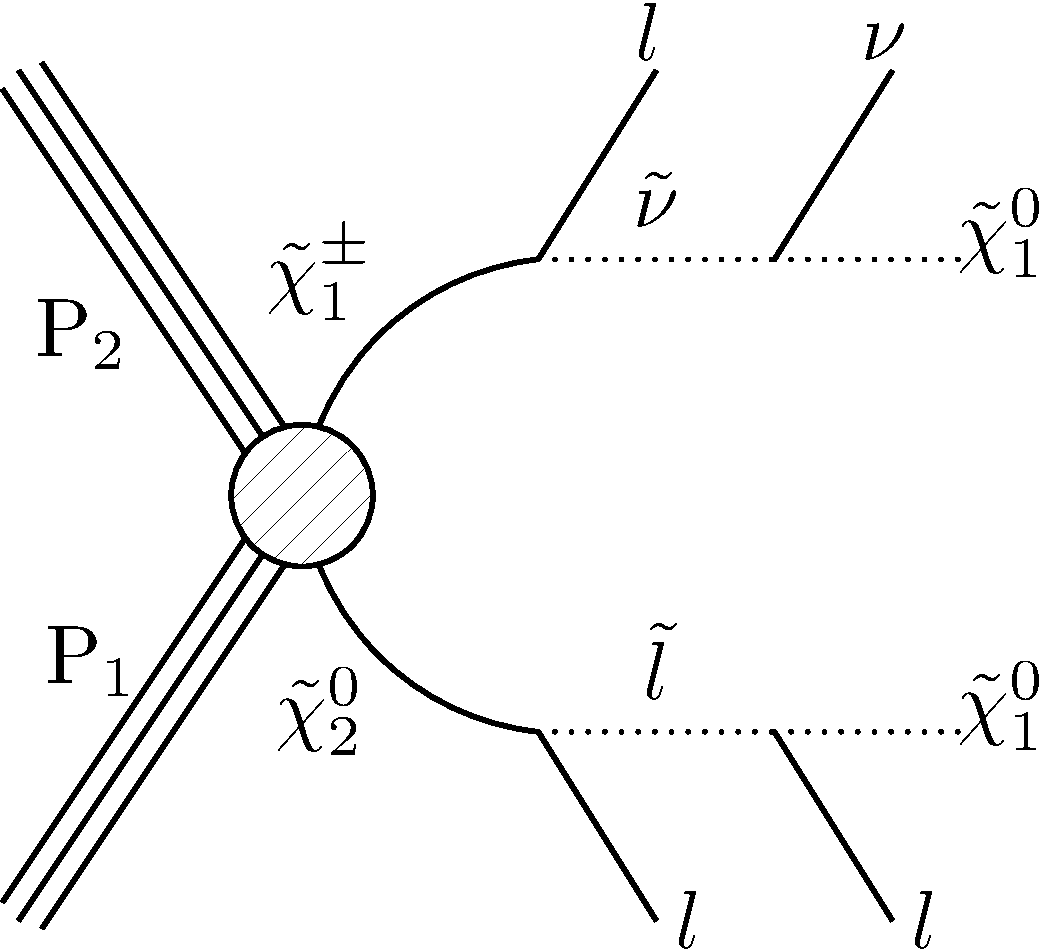
\includegraphics[width=0.26\linewidth]{figures/TChiChipmSnuSlep_feyn.pdf}}\spacer \\
\end{tabular}
\caption{The simplified models used for weakino production. \fixme{Once we know what models we use, we redo this list.}}
\label{fig:weakinoSMSes}
\end{center}
\end{figure}



\begin{table}[h!]\centering
\begin{tabular}{|c|c|c|c|c|c|}
\hline
additional & & & & & Results \\
particle content & Production & Decay & SMS & Figure & from \\
\hline
WZ & $\chipm\rightarrow W\chiz$ & & \model{TChiwz} & Fig.~\ref{fig:TChiwz} & multi leptons, \\
 & $\chitz \rightarrow Z\chiz$ & & & & comb. leptons \\
\hline
lll & $\chipm\rightarrow l \nu\chiz$ & & \model{TChiN2C1} & Fig.~\ref{fig:TChiN2C1} & multi leptons, \\
 & $\chitz \rightarrow ll\chiz$ & & & & comb. leptons \\
\hline
ZZ & $\chitz \rightarrow Z\chiz$ & & \model{TChizz} & Fig.~\ref{fig:TChizz} & ... \\
\hline
$\slep\slep$lll & $\chipm\rightarrow \nu\slep, $ & $\slep\rightarrow l\chiz$ & \model{TChiChipm-} & Fig.~\ref{fig:TChiChipmSlepSlep} & multi leptons, \\
 & $\chitz \rightarrow l\slep$ & & \model{SlepSlep} & & comb. leptons \\
\hline
$\slep\snu$lll  & $\chipm\rightarrow l\snu, \chitz \rightarrow l\slep$ & $\slep\rightarrow l\chiz$  & \model{TChiChipm-} & Fig.~\ref{fig:TChiChipmSnuSlep} & multi leptons, \\
 & & $\snu\rightarrow \nu\chiz$  & \model{SnuSlep} & & comb. leptons \\
\hline
\end{tabular}
\caption{SMS case ``weakinos'': Classification of events with charginos or neutralinos as SUSY mothers. Add TChiN2C1 et al.}
\label{tab:classweakinos}
\end{table}

\FloatBarrier

\subsection{Decomposing a pMSSM point -- an example}
\label{ssec:decomposeexample}
\fixme{I am only starting this section.} \\

Point 5jc0G1ixS2wq98jT76e8ieLS73LcJSWAE5FGb2ZFwUqx7xY6
\begin{figure}[ht!]
\begin{center}
\begin{tabular}{lc}
\subfigure[\label{fig:ruler}ruler plot, masses are given in GeV.]
{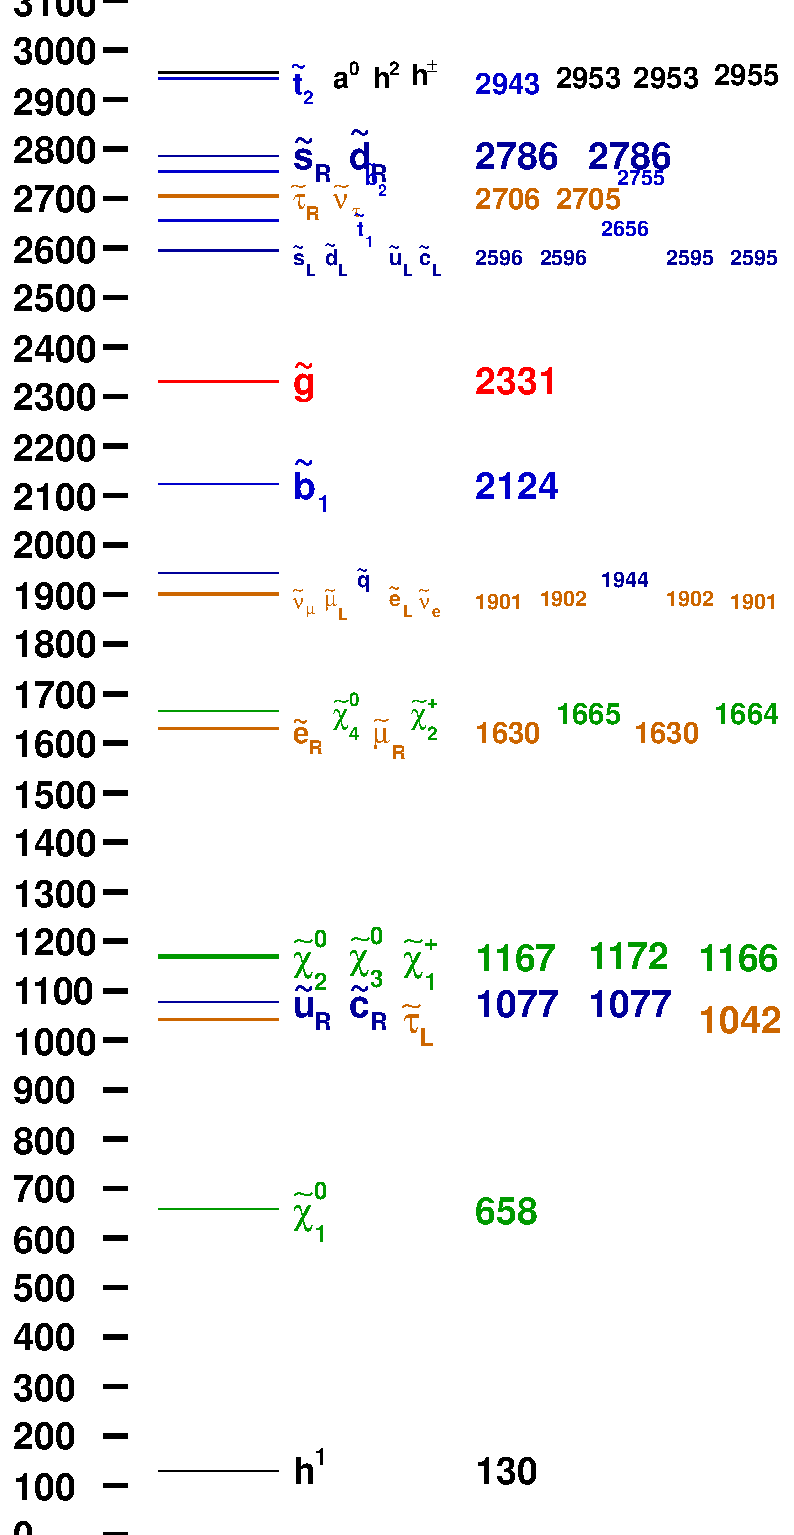
\includegraphics[width=0.26\linewidth]{figures/ruler.pdf}}\spacer &
\subfigure[\label{fig:decayplot}decay plot]{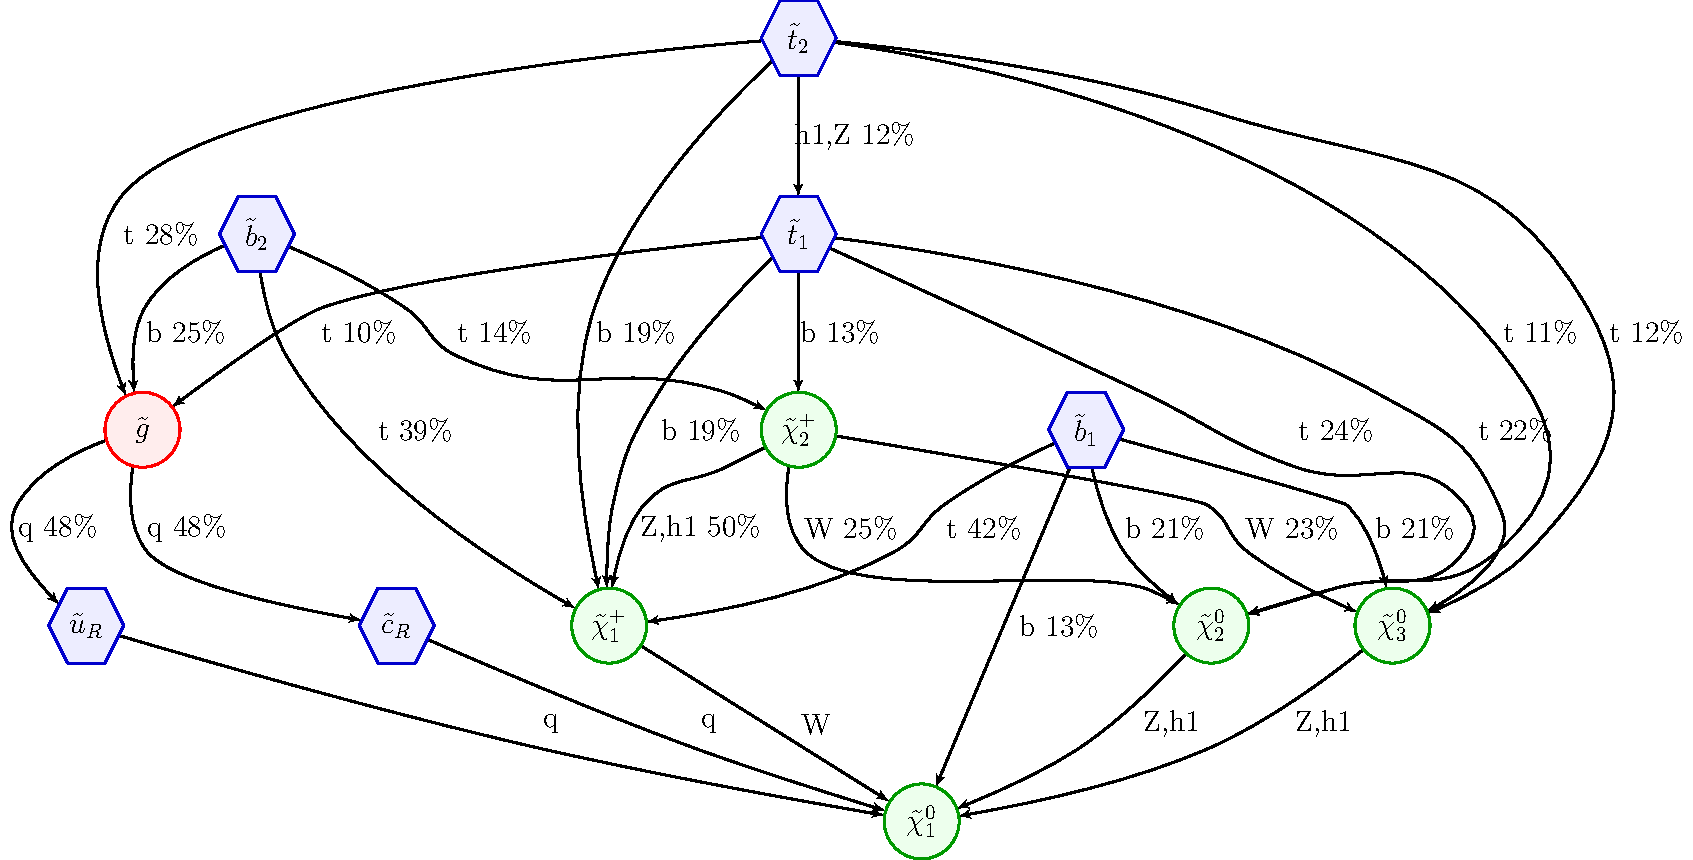
\includegraphics[width=0.72\linewidth]{figures/decay.pdf}}
\end{tabular}
\caption{ \fixme{Starting to add plots that show the decomposition.}}
\label{fig:decompositionexample}
\end{center}
\end{figure}

Blahblah walkding: \\
\url{http://www.hephy.at/user/walten/cgi-bin/pmssm.py?\\key=5jc0G1ixS2wq98jT76e8ieLS73LcJSWAE5FGb2ZFwUqx7xY6}
\FloatBarrier

